\documentclass[fleqn, a4paper, 11pt, oneside]{amsart}
%\usepackage[top = 2cm, bottom = 1cm, left = 1cm, right = 1cm]{geometry}
\usepackage{exsheets, tasks}
\usepackage{amsmath, amssymb, amsthm} %standard AMS packages
\usepackage{marginnote} %marginnotes
\usepackage{gensymb} %miscellaneous symbols
\usepackage{commath} %differential symbols
\usepackage{xcolor} %colours
\usepackage{cancel} %cancelling terms
\usepackage[free-standing-units, space-before-unit]{siunitx} %formatting units
\usepackage{tikz, pgfplots} %diagrams
\usetikzlibrary{calc, hobby, patterns, intersections, decorations.markings}
\usepackage{graphicx} %inserting graphics
\usepackage{hyperref} %hyperlinks
\usepackage{datetime} %date and time
\usepackage{ulem} %underline for \emph{}
\usepackage{xfrac} %inline fractions
\usepackage{enumerate,enumitem} %numbered lists
\usepackage{float} %inserting floats
\usepackage{circuitikz}[american voltages, american currents] %circuit diagrams

\newcommand\numberthis{\addtocounter{equation}{1}\tag{\theequation}} %adds numbers to specific equations in non-numbered list of equations

\newcommand{\AxisRotator}[1][rotate=0]{
	\tikz [x=0.25cm,y=0.60cm,line width=.2ex,-stealth,#1] \draw (0,0) arc (-150:150:1 and 1);%
} %rotation symbols on axes

\theoremstyle{definition}
\newtheorem{example}{Example}
\newtheorem{definition}{Definition}

\theoremstyle{theorem}
\newtheorem{theorem}{Theorem}

\newcommand{\curl}{\mathrm{curl\,}}

\makeatletter
\@addtoreset{section}{part} %resets section numbers in new part
\makeatother

\renewcommand{\thesubsection}{(\arabic{subsection})}
\renewcommand{\thesection}{(\arabic{section})}

%section headings on left
\makeatletter
\def\specialsection{\@startsection{section}{1}%
	\z@{\linespacing\@plus\linespacing}{.5\linespacing}%
	%  {\normalfont\centering}}% DELETED
	{\normalfont}}% NEW
\def\section{\@startsection{section}{1}%
	\z@{.7\linespacing\@plus\linespacing}{.5\linespacing}%
	%  {\normalfont\scshape\centering}}% DELETED
	{\normalfont\scshape}}% NEW
\makeatother

%forces newline after subsection
\makeatletter
\def\subsection{\@startsection{subsection}{3}%
	\z@{.5\linespacing\@plus.7\linespacing}{.1\linespacing}%
	{\normalfont\itshape}}
\makeatother

\settasks{counter-format = tsk[1].}

\SetupExSheets{solution/print = true}

%opening
\title{Quantum and Solid State Physics : Assignment 1}
\author
{
	Aakash Jog\\
	ID : 989323563
}
\date{\formatdate{22}{10}{2015}}

\begin{document}

\tikzset{->-/.style={decoration={
  markings,
  mark=at position #1 with {\arrow{>}}},postaction={decorate}}}

\maketitle
%\setlength{\mathindent}{0pt}

\begin{question}
	List some common semiconductors: elemental, binary($\mathrm{III}$-$\mathrm{V}$ and $\mathrm{II}$-$\mathrm{VI}$), and ternary($\mathrm{III}$-$\mathrm{V}$).
	Look up their energy band gaps and list them in the table.
\end{question}

\begin{solution}
	\begin{table}[H]
		\begin{tabular}{|l|l|}
			\hline
			Elemental Semiconductors: Group $\mathrm{IV}$ & Energy Band Gap (\si{\electronvolt}) \\
			\hline
			Si                                            & 1.1                                  \\
			Ge                                            & 0.66                                 \\
			\hline
		\end{tabular}
	\end{table}
	\begin{table}[H]
		\begin{tabular}{|l|l|}
			\hline
			Binary Semiconductors: $\mathrm{II}$-$\mathrm{VI}$ & Energy Band Gap (\si{\electronvolt}) \\
			\hline
			CdSe                                               & 1.74                                 \\
			CdTe                                               & 1.44                                 \\
			ZnO                                                & 3.2                                  \\
			ZnS                                                & 3.6                                  \\
			\hline
		\end{tabular}
	\end{table}
	\begin{table}[H]
		\begin{tabular}{|l|l|}
			\hline
			Binary Semiconductors: $\mathrm{III}$-$\mathrm{V}$ & Energy Band Gap (\si{\electronvolt}) \\
			\hline
			InSb                                               & 0.17                                 \\
			InAs                                               & 0.36                                 \\
			InP                                                & 1.27                                 \\
			GaN                                                & 3.4                                  \\
			GaAs                                               & 1.43                                 \\
			AlAs                                               & 2.12                                 \\
			GaP                                                & 2.25                                 \\
			GaSb                                               & 0.68                                 \\
			\hline
		\end{tabular}
	\end{table}
\end{solution}

\begin{question}
	\begin{enumerate}
		\item
			Suppose a photo is emitted from a semiconductor device with energy equal to the energy band gap of GaN, i.e. $E_{\textnormal{photon}} = E_{\textnormal{gap, GaN}}$.
			What is the wavelength of light, in \si{\micro\metre}, that is emitted?
			Would we be able to observe the light emitted?
			If so, what colour of light may be emitted?
		\item
			Repeat the above for photon energy equal to the energy band gap of GaAs.
	\end{enumerate}
\end{question}

\begin{solution}
	\begin{enumerate}[leftmargin=*]
		\item
			\begin{align*}
				E                  & = \frac{h c}{\lambda}                                                 \\
				\therefore \lambda & = \frac{h c}{E}                                                       \\
                                                   & = \frac{1.24 \si{\electronvolt \micro\metre}}{3.4 \si{\electronvolt}} \\
                                                   & = 0.365 \si{\micro\metre}                                             \\
                                                   & = 365 \si{\nano\metre}
			\end{align*}
			Therefore, the wavelength of the light emitted is in the visible range, and the colour of the light emitted will be violet.
		\item
			\begin{align*}
				E                  & = \frac{h c}{\lambda}                                                  \\
				\therefore \lambda & = \frac{h c}{E}                                                        \\
                                                   & = \frac{1.24 \si{\electronvolt \micro\metre}}{1.43 \si{\electronvolt}} \\
                                                   & = 0.867 \si{\micro\metre}                                              \\
                                                   & = 867 \si{\nano\metre}
			\end{align*}
			Therefore, the wavelength of the light emitted is not in the visible range.
	\end{enumerate}
\end{solution}

\begin{question}
	Derive the resistance $R$ of the following material structure, in terms of its electrical conductivity $\sigma$ and dimensions shown below.
	\begin{figure}[H]
		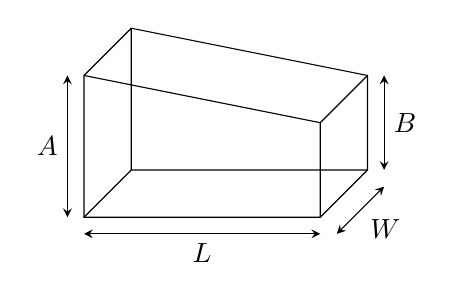
\begin{tikzpicture}[scale = 0.6]
			\def\A{3};
			\def\L{5};
			\def\B{2};
			\def\W{1};

			\begin{scope}
				\draw (0,0) -- (\L,0) -- (\L,\B) -- (0,\A) -- cycle;
				\draw [xshift = \W cm, yshift = \W cm] (0,0) -- (\L,0) -- (\L,\B) -- (0,\A) -- cycle;

				\draw (0,0) -- ++(\W,\W);
				\draw (\L,0) -- ++(\W,\W);
				\draw (\L,\B) -- ++(\W,\W);
				\draw (0,\A) -- ++(\W,\W);
			\end{scope}

			\begin{scope}[stealth-stealth]
				\draw [xshift = -10] (0,0) -- (0,\A) node [midway, left] {$A$};
				\draw [yshift = -10] (0,0) -- (\L,0) node [midway, below] {$L$};
				\draw [xshift = 10] ($ (\L,0) + (\W,\W) $) -- ($ (\L,\B) + (\W,\W) $) node [midway, right] {$B$};
				\draw [xshift = 10, yshift = -10] (\L,0) -- ++(\W,\W) node [midway, below right] {$W$};
			\end{scope}
		\end{tikzpicture}
	\end{figure}
\end{question}

\begin{solution}
	Consider a slice with height $h$, width $w$, and thickness $\dif x$.
	Therefore, the cross-sectional area of the elemental slice is
	\begin{align*}
		\dif A & = w h \\
                       & = w \left( \frac{A - B}{L} x + A \right)
	\end{align*}
	Let the resistance of the elemental slice be $\dif R$.\\
	Therefore,
	\begin{align*}
		\dif R       & = \frac{\dif x}{\sigma w h}                                                                 \\
                             & = \frac{\dif x}{\sigma w \left( \frac{B - A}{L} x + A \right)}                              \\
                             & = \frac{1}{\sigma w} \frac{\dif x}{\frac{B - A}{L} x + A}                                   \\
		\therefore R & = \frac{1}{\sigma w} \int\limits_{0}^{L} \frac{\dif x}{\frac{B - A}{L} x + A}               \\
                             & = \frac{L}{\sigma w} \int\limits_{0}^{L} \frac{\dif x}{(B - A) x + A L}                     \\
                             & = \frac{L}{\sigma w} \left. \frac{\ln\left( (B - A) x + A L \right)}{B - A} \right|_{0}^{L} \\
                             & = \frac{L}{\sigma w} \left( \frac{\ln(B L)}{B - A} - \frac{\ln(A L)}{B - A} \right)         \\
                             & = \frac{L}{\sigma w} \left( \frac{\ln\left( \frac{B}{A} \right)}{B - A} \right)
	\end{align*}
\end{solution}

\begin{question}
	In early experiments to investigate the photoelectric effect, a beam of light of a single frequency was directed at a clean surface of potassium metal.
	The maximum kinetic energy of electrons which were ejected from the metal was measured.
	When the experiment was repeated with different frequencies of light, the maximum kinetic energy of electrons depended on the frequency of the light as shown below.
	\begin{figure}[H]
		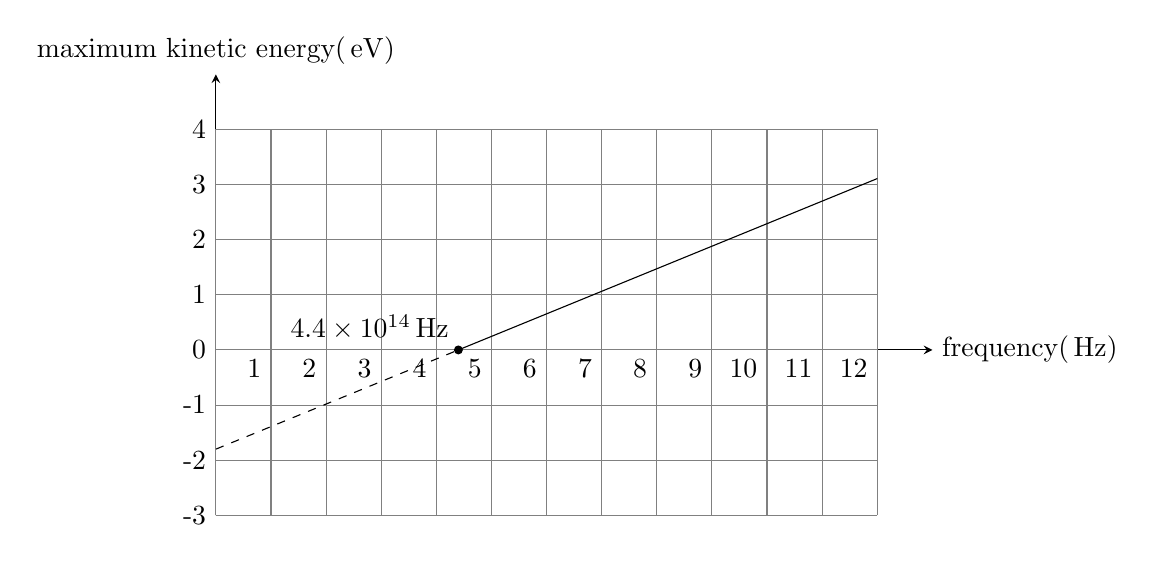
\begin{tikzpicture}[scale = 0.7]
			\begin{scope}[-stealth]
				\draw (0,-3) -- (0,5) node [above] {maximum kinetic energy(\electronvolt)};
				\draw (0,0) -- (13,0) node [right] {frequency(\hertz)};
			\end{scope}

			\draw [gray] (0,-3) grid (12,4);

			\foreach \y in {-3,-2,-1,0,1,2,3,4}
			{
				\node [left] at (0,\y) {\y};
			}

			\foreach \x in {1,...,12}
			{
				\node [below left] at (\x,0) {\x};
			}

			\clip (0,-3) rectangle (12,4);

			\draw [dashed] (0,-1.8) -- (4.4,0);
			\draw (4.4,0) -- ++(8.8,3.6);

			\filldraw (4.4,0) circle (2pt) node [above left] {$4.4 \times 10^{14} \hertz$};
		\end{tikzpicture}
	\end{figure}
	What is the minimum energy of an incident photon, in \electronvolt, that can eject an electron from potassium metal?
\end{question}

\begin{solution}
	The frequency of the incident photon, which corresponds to the maximum kinetic energy of the ejected electron being zero, is $4.4 \times 10^{14} \hertz$.\\
	The energy of this photon is the minimum energy required to eject an electron.\\
	Therefore, the minimum energy capable of ejecting a photon from potassium is
	\begin{align*}
		E & = h \nu                                                                               \\
                  & = (4.136 \times 10^{-15} \si{\electronvolt \second}) (4.4 \times 10^{14} \si{\hertz}) \\
                  & = 18.1984 \si{\electronvolt}
	\end{align*}
\end{solution}

\begin{question}
	The minimum photon energy required to eject electrons from copper is approximately double the value for potassium.
	\begin{enumerate}
		\item
			Which of the graphs below would best describe the results if the experiment were repeated with copper instead of potassium?
			Explain you choice, commenting on the slope of the lines for potassium and copper, and the points where the lines cross the frequency axis.
			\begin{enumerate}
				\item
					~\\
					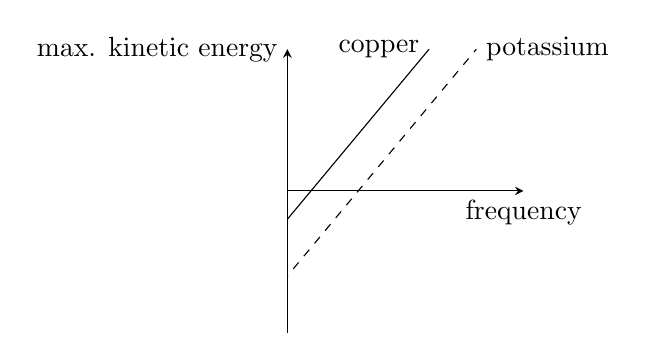
\begin{tikzpicture}[scale = 0.6]
						\begin{scope}[-stealth]
							\draw (0,0) -- (5,0) node [below] {frequency};
							\draw (0,-3) -- (0,3) node [left] {max. kinetic energy};
						\end{scope}
						\begin{scope}
							\clip (0,-3) rectangle (5,3);

							\draw (-2,-3) -- (3,3);
							\draw [dashed] (-1,-3) -- (4,3);
						\end{scope}
						\begin{scope}
							\node [left] at (3,3) {copper};
							\node [right] at (4,3) {potassium};
						\end{scope}
					\end{tikzpicture}
				\item
					~\\
					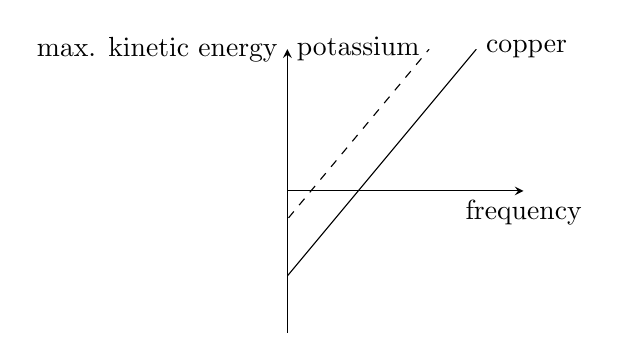
\begin{tikzpicture}[scale = 0.6]
						\begin{scope}[-stealth]
							\draw (0,0) -- (5,0) node [below] {frequency};
							\draw (0,-3) -- (0,3) node [left] {max. kinetic energy};
						\end{scope}
						\begin{scope}
							\clip (0,-3) rectangle (5,3);

							\draw [dashed] (-2,-3) -- (3,3);
							\draw (-1,-3) -- (4,3);
						\end{scope}
						\begin{scope}
							\node [left] at (3,3) {potassium};
							\node [right] at (4,3) {copper};
						\end{scope}
					\end{tikzpicture}
				\item
					~\\
					\begin{tikzpicture}[scale = 0.6]
						\begin{scope}[-stealth]
							\draw (0,0) -- (5,0) node [below] {frequency};
							\draw (0,-3) -- (0,3) node [left] {max. kinetic energy};
						\end{scope}
						\begin{scope}
							\clip (0,-3) rectangle (5,3);

							\draw (0,-2) -- (3,4);
							\draw [dashed] (0,-1) -- (5,4);
						\end{scope}
						\begin{scope}
							\node [left] at (3,4) {copper};
							\node [right] at (5,4) {potassium};
						\end{scope}
					\end{tikzpicture}
				\item
					~\\
					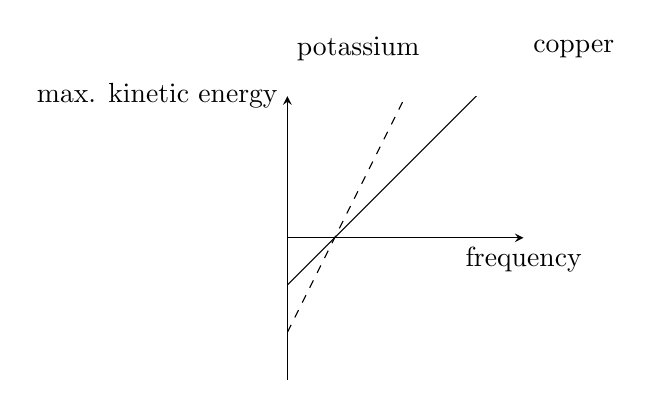
\begin{tikzpicture}[scale = 0.6]
						\begin{scope}[-stealth]
							\draw (0,0) -- (5,0) node [below] {frequency};
							\draw (0,-3) -- (0,3) node [left] {max. kinetic energy};
						\end{scope}
						\begin{scope}
							\clip (0,-3) rectangle (5,3);

							\draw [dashed] (0,-2) -- (3,4);
							\draw (0,-1) -- (5,4);
						\end{scope}
						\begin{scope}
							\node [left] at (3,4) {potassium};
							\node [right] at (5,4) {copper};
						\end{scope}
					\end{tikzpicture}
			\end{enumerate}
		\item
			When ultraviolet light is incident on a sample of potassium, electrons are emitted from the surface of the metal.
			The kinetic energy of the most energetic electrons emitted is found to be dependent upon the frequency of the radiation used, as shown in the graph below.
			\begin{figure}[H]
				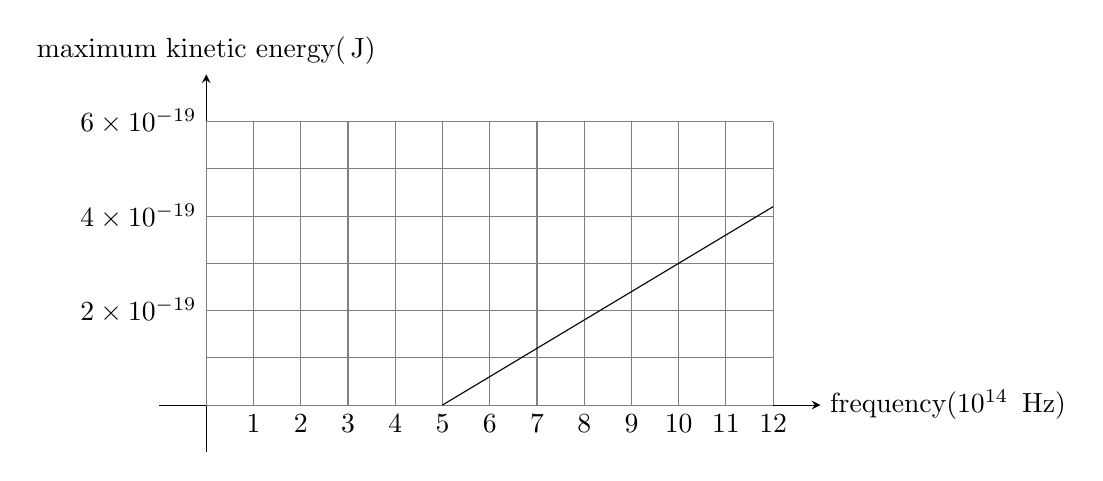
\begin{tikzpicture}[scale = 0.6]
					\begin{scope}[-stealth]
						\draw (0,-1) -- (0,7) node [above] {maximum kinetic energy(\joule)};
						\draw (-1,0) -- (13,0) node [right] {frequency($10^{14}$ \hertz)};
					\end{scope}
		
					\draw [gray] (0,0) grid (12,6);
		
					\foreach \y in {2,4,6}
					{
						\node [left] at (0,\y) {$\y \times 10^{-19}$};
					}
		
					\foreach \x in {1,...,12}
					{
						\node [below] at (\x,0) {\x};
					}
		
					\clip (0,0) rectangle (12,6);
		
					\draw (5,0) -- (15,6);
				\end{tikzpicture}
			\end{figure}
			Which of the graphs below represents the result if the intensity of the light were doubled?
			Which one or more of the graphs below could represent the result if the potassium were replaced by another metal?
			\begin{enumerate}
				\item
					~\\
					\begin{figure}[H]
						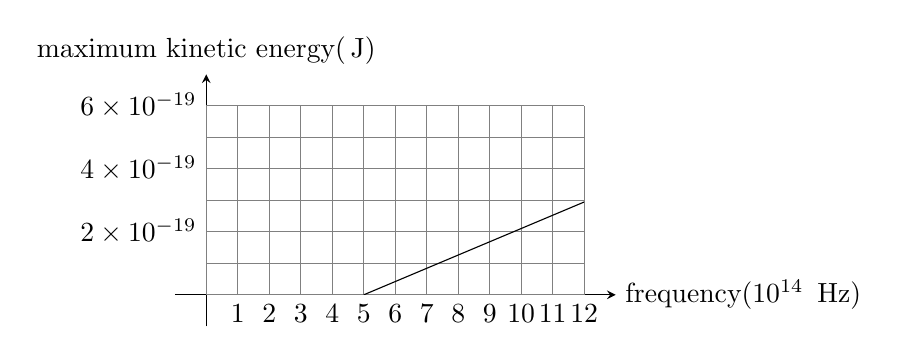
\begin{tikzpicture}[scale = 0.4]
							\begin{scope}[-stealth]
								\draw (0,-1) -- (0,7) node [above] {maximum kinetic energy(\joule)};
								\draw (-1,0) -- (13,0) node [right] {frequency($10^{14}$ \hertz)};
							\end{scope}
				
							\draw [gray] (0,0) grid (12,6);
				
							\foreach \y in {2,4,6}
							{
								\node [left] at (0,\y) {$\y \times 10^{-19}$};
							}
				
							\foreach \x in {1,...,12}
							{
								\node [below] at (\x,0) {\x};
							}
				
							\clip (0,0) rectangle (12,6);
				
							\draw (5,0) -- (24,8);
						\end{tikzpicture}
					\end{figure}
				\item
					~\\
					\begin{figure}[H]
						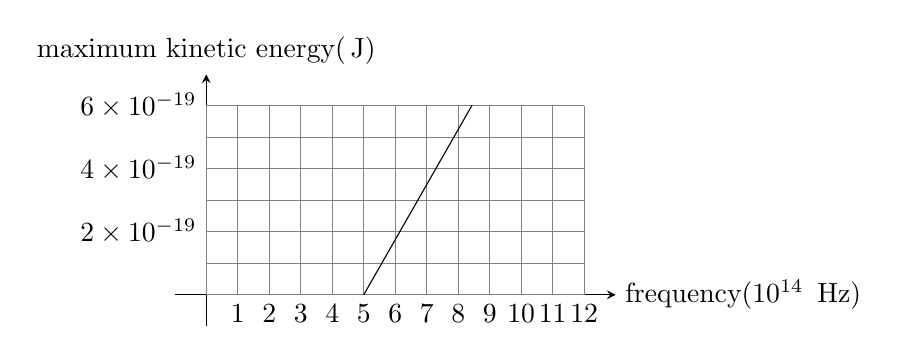
\begin{tikzpicture}[scale = 0.4]
							\begin{scope}[-stealth]
								\draw (0,-1) -- (0,7) node [above] {maximum kinetic energy(\joule)};
								\draw (-1,0) -- (13,0) node [right] {frequency($10^{14}$ \hertz)};
							\end{scope}
				
							\draw [gray] (0,0) grid (12,6);
				
							\foreach \y in {2,4,6}
							{
								\node [left] at (0,\y) {$\y \times 10^{-19}$};
							}
				
							\foreach \x in {1,...,12}
							{
								\node [below] at (\x,0) {\x};
							}
				
							\clip (0,0) rectangle (12,6);
				
							\draw (5,0) -- (9,7);
						\end{tikzpicture}
					\end{figure}
				\item
					~\\
					\begin{figure}[H]
						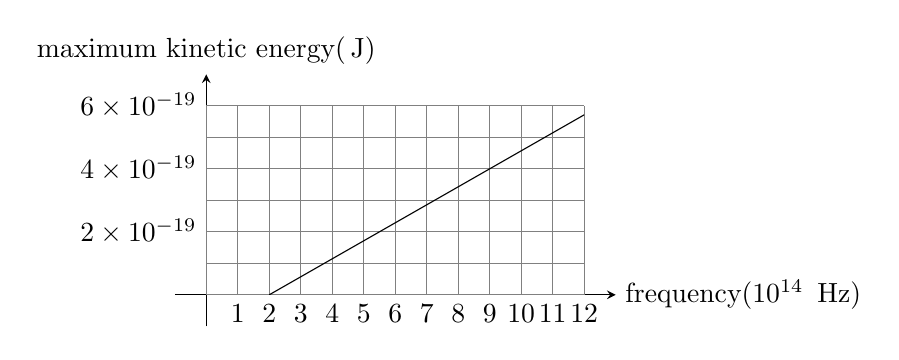
\begin{tikzpicture}[scale = 0.4]
							\begin{scope}[-stealth]
								\draw (0,-1) -- (0,7) node [above] {maximum kinetic energy(\joule)};
								\draw (-1,0) -- (13,0) node [right] {frequency($10^{14}$ \hertz)};
							\end{scope}
				
							\draw [gray] (0,0) grid (12,6);
				
							\foreach \y in {2,4,6}
							{
								\node [left] at (0,\y) {$\y \times 10^{-19}$};
							}
				
							\foreach \x in {1,...,12}
							{
								\node [below] at (\x,0) {\x};
							}
				
							\clip (0,0) rectangle (12,6);
				
							\draw (2,0) -- (16,8);
						\end{tikzpicture}
					\end{figure}
				\item
					~\\
					\begin{figure}[H]
						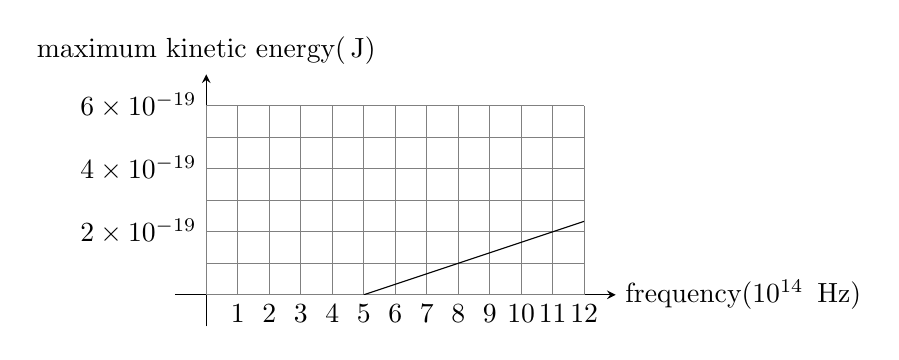
\begin{tikzpicture}[scale = 0.4]
							\begin{scope}[-stealth]
								\draw (0,-1) -- (0,7) node [above] {maximum kinetic energy(\joule)};
								\draw (-1,0) -- (13,0) node [right] {frequency($10^{14}$ \hertz)};
							\end{scope}
				
							\draw [gray] (0,0) grid (12,6);
				
							\foreach \y in {2,4,6}
							{
								\node [left] at (0,\y) {$\y \times 10^{-19}$};
							}
				
							\foreach \x in {1,...,12}
							{
								\node [below] at (\x,0) {\x};
							}
				
							\clip (0,0) rectangle (12,6);
				
							\draw (5,0) -- (14,3);
						\end{tikzpicture}
					\end{figure}
				\item
					~\\
					\begin{figure}[H]
						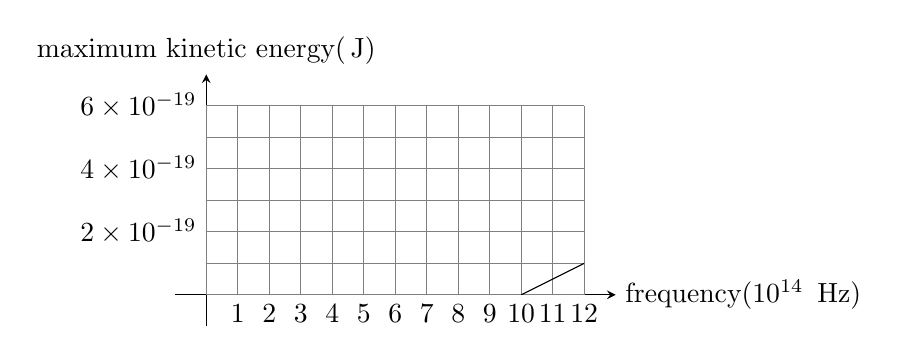
\begin{tikzpicture}[scale = 0.4]
							\begin{scope}[-stealth]
								\draw (0,-1) -- (0,7) node [above] {maximum kinetic energy(\joule)};
								\draw (-1,0) -- (13,0) node [right] {frequency($10^{14}$ \hertz)};
							\end{scope}
				
							\draw [gray] (0,0) grid (12,6);
				
							\foreach \y in {2,4,6}
							{
								\node [left] at (0,\y) {$\y \times 10^{-19}$};
							}
				
							\foreach \x in {1,...,12}
							{
								\node [below] at (\x,0) {\x};
							}
				
							\clip (0,0) rectangle (12,6);
				
							\draw (10,0) -- (14,2);
						\end{tikzpicture}
					\end{figure}
			\end{enumerate}
	\end{enumerate}
\end{question}

\begin{solution}
	\begin{enumerate}
		\item
			As the minimum energy required to eject an electron from copper is double that of the minimum energy required to eject an electron from potassium, the intersection of the graph of copper, with the frequency axis, must be to the right of that of potassium.\\
			After the threshold frequency, the maximum kinetic energy of the ejected electron is independent of any property of the metal.
			Therefore, the slopes of the two graphs are equal.\\
			Hence, the correct graph is the second one.
		\item
			The kinetic energy of the ejected electron is dependent only on the frequency of the incident photons, and not dependent on the intensity of the light.
			Therefore, even if the intensity were doubled, the graph would be identical.
			Hence, the correct graph is the first one.\\
			~\\
			If potassium were replaced by another metal, the only quantity that would change is the cutoff frequency.
			Therefore, the third graph represents the result if potassium were replaced by another metal.
	\end{enumerate}
\end{solution}

\end{document}
